\chapter{Implementierung}

	In diesem Kapitel werden einige Implementationsdetails dargestellt und erläutert, welche entweder einen kritischen Aspekt des Projekts darstellen oder von hoher Relevanz für den Erfolg des Projektes sind. 
	
	\section{Controller Interfaces}
	
		Wie bereits erwähnt sind die sog. Controller in einer \acs{MVC} Architektur für den Behandlung von Benutzereingaben zuständig. Im Falle einer \acs{REST}ful \acs{API} -- hier durch Spring umgesetzt -- dienen Controller dem Zweck, alle eingehenden \acs{HTTP} Anfragen zu behandeln. Dafür bietet Spring Annotationen, mit dessen Hilfe eindeutig definiert werden kann, wie die Anfrage auszusehen hat. Diese Definition eines sog. Endpoints beinhaltet immer einen Pfad, unter welchem der Endpoint erreicht werden kann, und eine \acs{HTTP} Methode. Es kann zusätzlich noch festgelegt werden, welche \acs{HTTP} Header bei einer Anfrage angegeben werden sollen und welcher \acs{MIME} Type zurück gegeben wird.
		
		\autoref{code:CityApi} zeigt beispielhaft, wie eine solche Definition eines Endpoints aussehen kann. Die eigentliche Beschreibung des Endpoints wird durch die Annotation \lstinline|@GetMapping| beschrieben. 	
		
		Um jedoch eine ausführlichere Beschreibung des Endpoints zu erstellen, können die von Swagger bereitgestellten Annotation verwendet werden. So lassen sich beispielsweise die Parameter, die Rückgabewerte aber auch die Authentifizierungsmethode beschreiben. Außerdem lassen sich noch Beschreibungen einfügen, um die Benutzung der \acs{API} zu erleichtern und zu dokumentieren. Für die City \acs{API} wird ein String als Parameter benötigt, mit dessen Hilfe die entsprechende Stadt zurückgegebene werden kann. Außerdem wird ein \acs{API} Key benötigt, um sich zu authentifizieren. 
		
		\lstinputlisting[
			label=code:CityApi,
			caption=Nutzung der beschriebenen Annotationen eines Controllers am Beispiel der City API,
			captionpos=b,               % Position, an der die Caption angezeigt wird t(op) oder b(ottom)
			style=EigenerJavaStyle,     % Eigener Style der vor dem Dokument festgelegt wurde
		]{code/CityApi.java}
		
	\section{Authentifizierung}
	
		\begin{figure}[ht!]
			\centering
			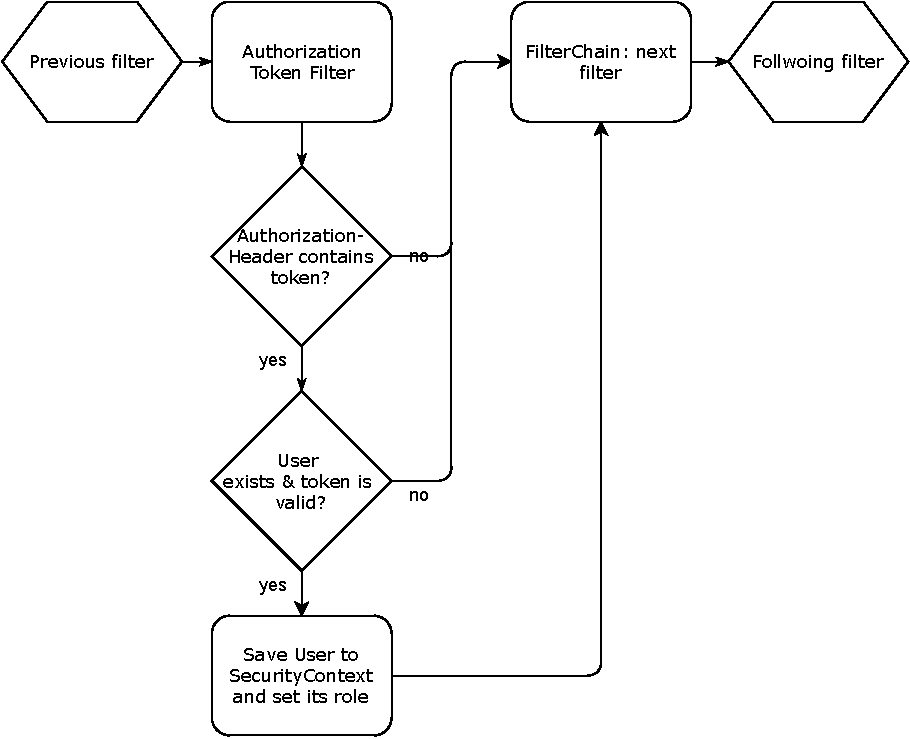
\includegraphics[width=1\textwidth]{images/authorization-flow-chart.pdf}
			\caption{Authentifizierungsprozess von \textit{Travlyn} mittels Spring Security Filter Chain}
			\label{fig:authenticationProcess}
		\end{figure} 
		
		\textit{Travlyn} stellt insgesamt zwei verschiedene Authentifizierungsrollen bereit. Wie \autoref{fig:UCD} zeigt, gibt es zum einen die Rolle des \acs{API}-Benutzers und die des registrierten Benutzers. Dem API Benutzer ist es erlaubt, Informationen wie beispielsweise über Trips anzufragen, wohingegen ein registrierter Benutzer auch die Möglichkeit hat, einen Trip zu erstellen. 
		
		Der Prozess der Authentifizierung basiert bei \textit{Travlyn} auf sog. Tokens. Sobald sich ein Benutzer registriert oder anmeldet, wird ein Token generiert -- das Token besteht aus 32 Zeichen und Ziffern und besitzt zudem ein Ablaufdatum, welches bei Überschreiten das Token als ungültig gekennzeichnet --, auf der Datenbank abgespeichert und zurück an den Benutzer gesendet. Um nun Endpoints anzufragen, welche eine Authentifizierung benötigen, wird dieses Token im \lstinline|Authorization|-Header im Format \lstinline|Bearer <token string>| gesendet. Auf dem Server erfolgt nun die Validierung des Tokens. So kann außerdem festgestellt werden, wer eine bestimmte Aktion ausgeführt hat. 
		
		Spring stellt für diesen Prozess einen Mechanismus bereit, um diese Authentifizierung möglichst einfach umzusetzen: Bevor eine Anfrage an einen bestimmten Endpoint zugelassen und die entsprechende Controller-Methode (wie bei \autoref{code:CityApi} beispielhaft gezeigt) aufgerufen wird, durchläuft diese Anfrage eine Reihe von Filtern. Diese sog. Filter Chain beinhaltet unter Anderem auch Authentifizierungsmechanismen, die sich eigens definieren lassen. So wurde für \textit{Travlyn} ein Filter namens \lstinline|AuthenticationTokenFilter| entwickelt, der dazu dient, das Token aus dem \acs{HTTP}-Header zu extrahieren und zu validieren. 
		
		Wenn das Token valide ist und auch der korrekten Benutzerrolle -- \acs{API}- oder registrierter Nutzer -- zugeordnet werden kann, wird die Anfrage an die entsprechende Controller Methode weitergeleitet und der entsprechende Nutzer im sog. \lstinline|SecurityContext| gespeichert, sodass auf die Rolle des Benutzers und auch auf den Benutzer selbst beim Prozessieren der Anfrage zugegriffen werden kann. Ist dies nicht der Fall, so wird diese Anfrage als nicht-authentifiziert markiert. \autoref{fig:authenticationProcess} visualisiert den Authentifizierungsprozess, wie er bei \textit{Travlyn} umgesetzt wurde.
		
		Um die zugelassenen Benutzerrollen für einen Endpoint der \acs{API} festzulegen, stellt das Modul Spring Security unter anderem die Annotation \lstinline|@PreAuthorize| zur Verfügung. Als Parameter wird ein in der \ac{SpEL} geschriebener Ausdruck übergeben, wie beispielsweise \lstinline|hasRole(API_USER)| in \autoref{code:CityApi}. So lässt sich die gesendete Authentisierung des Benutzers automatisiert überprüfen.
		
	\section{Namenzuordnung zwischen den \acs{API}s}
	
	(Joshua)
	
	Wie in \autoref{sec:datengrundlage} beschrieben werden für \textit{Travlyn} mehrere verschiedene \acs{API}s benutzt um alle relevanten Informationen zusammen zu sammeln. Leider ergeben sich bei einer derartigen Parallelbenutzung häufig Inkompatibilitäten, grade wenn die \acs{API}s nicht von dem selben Anbieter stammen.
	
	\vspace{0.25cm}
	
	Im Fall von \textit{Travlyn} besteht eine solche Inkompatibilität zwischen der OpenRouteService \acs{API}, welche die Positionen und Namen der \acs{POI}s liefert und der DBpedia \acs{API}, welche die entsprechenden Informationen von Wikipedia bezieht: OpenRouteService liefert die Namen der Punkte in der Landessprache z.B. \enquote{Schloss Karlsruhe}. Dem gegenüber können bei DBpedia nur englische Namen abgefragt werden, wie z.B. \enquote{Karlsruhe Palace}. Des weiteren stehen selbst in englischsprachigen Ländern einige Namen in Konflikt wie z.B. \enquote{Coca Cola London Eye} auf \acs{ORS} zu \enquote{London Eye} auf DBpedia. Durch diese Konflikte fehlen viele Infos in der \textit{Travlyn} App und müssen manuell nachgepflegt werden.
	
	\vspace{0.25cm}
	
	Da diese Arbeit nicht darauf ausgelegt ist eine zur Veröffentlichung bereite App zu erstellen, sondern Konzepte und Wege aufzuzeigen, welche verwendet werden können wurde diese Nachpflege lediglich für einige Sehenswürdigkeiten in Karlsruhe durchgeführt und die entsprechende Infrastruktur für eine ausgedehntere Pflege geschaffen. Sollte die App produktiv veröffentlicht werden sind mehrere Möglichkeiten der Pflege vorstellbar: Es werden entsprechende Agenturen gebucht um die Zuordnung manuell in einer Datenbank zu pflegen und für möglichst viele Städte zur Verfügung zu stellen. Außerdem könnte auf einen Nutzerbasierten Ansatz gesetzt werden, bei dem die Nutzer die Möglichkeit haben Fehler und fehlende Infos nachzupflegen, sobald sie auffallen. Dies hätten den Vorteil, dass es für den Hersteller kostenlos ist und gut skaliert. Wahrscheinlich wäre eine Kombination aus beiden Möglichkeiten der beste Weg.
	
	\section{Umgehung der API Beschränkung für DBpedia}
	
	Der Umgang mit DBpedia für dieses Projekt wurde neben dem oben beschriebenen Mappingproblem auch durch die Abfragebeschränkung erschwert. Trotz einem registrierten persönlichen \acs{API} Schlüssels stehen der \textit{Travlyn} App nur 100 Abfragen pro Minute, 1000 Abfragen pro Stunde und 10000 Abfragen pro Tag zur Verfügung. 
	
	\vspace{0.25cm}
	
	Unter Betrachtung des Umstandes, dass jede neu abgefragte Stadt und jeder in dieser Stadt befindliche \acs{POI} abgefragt werden muss, wenn ein Nutzer sich per \textit{Travlyn} über eine Stadt informieren möchte, ist leicht zu erkennen, dass diese Beschränkung kaum eingehalten werden kann. Beispielsweise liefert \acs{ORS} für die Stadt London ca. 670 \acs{POI}s, die alle in einer für den Nutzer angemessenen Zeit abgefragt werden müssten. Dies kollidiert eindeutig mit der Minutenbeschränkung von DBpedia.
	Aus diesem Grund wurde für \textit{Travlyn} ein Konzept entwickelt, was ein \textit{lazy fetching} ermöglicht und die nötigen Abfragen erst nach und nach absetzt und den Nutzer möglichst wenig einschränkt:
	Für eine neue (nicht im Cache befindliche) Stadt wir sowohl die Abfrage für die Stadt als auch für bis zu 99 \acs{POI}s durchgeführt. Dies ist konform mit der Beschränkung von DBpedia und versucht den Nutzer möglichst wenig einzuschränken, indem die \acs{POI}s bevorzugt abgefragt werden, für die sich der aktuelle Nutzer laut seiner Präferenzen interessiert. Es wird eine entsprechend reduzierte Antwort an den Client geschickt, mit dem Hinweis, dass einige \acs{POI}s fehlen könnten. Nun hat der Nutzer die Möglichkeit, nach der Durchsicht der vorhandenen Sehenswürdigkeiten, weitere anzufordern und damit weitere Anfragen auf DBpedia auszulösen. Ebenso löst jede weitere Suche nach der vorliegenden Stadt weitere Requests aus. Dieses Verfahren operiert, bis alle \acs{POI}s abgefragt wurden. \autoref{fig:DBpediaFlow} zeigt vereinfacht den allgemeinen Ablauf des Verfahrens.
	
	\begin{figure}[ht!]
		\centering
		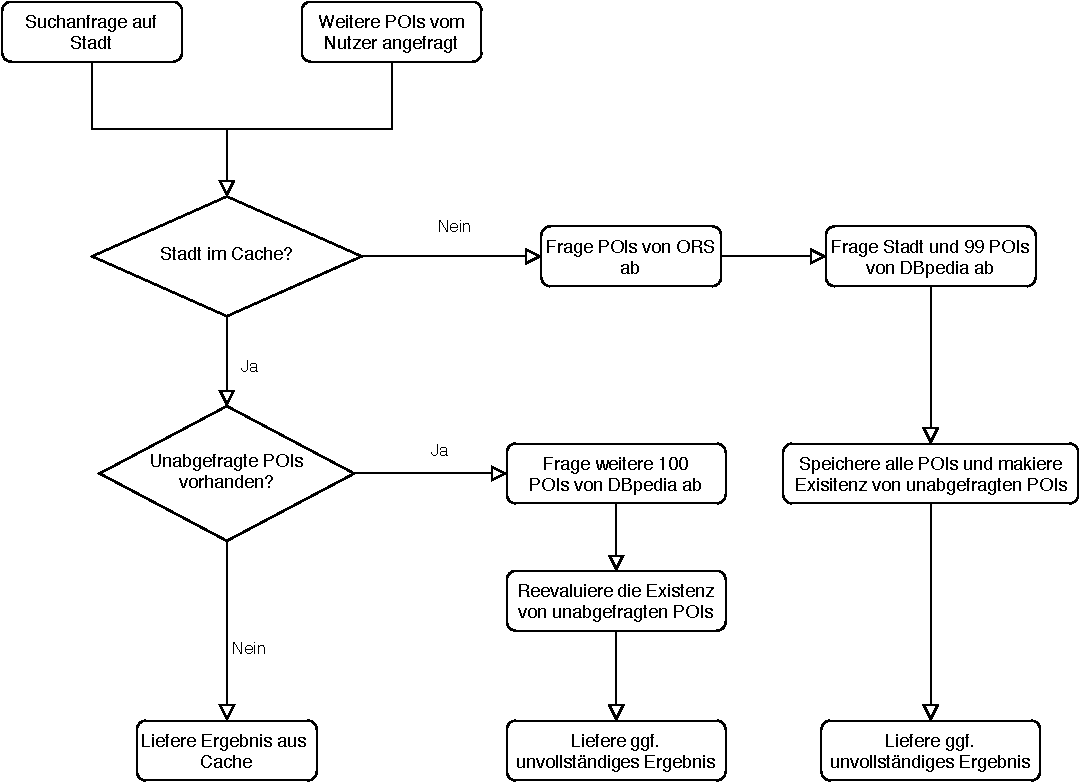
\includegraphics[width=1\textwidth]{images/DBpediaFlow.pdf}
		\caption{Flussdiagramm zum Ablauf des lazy fetching von DBpedia.}
		\label{fig:DBpediaFlow}
	\end{figure}

	Über diesen Mechanismus können die \enquote{burstartigen} Abfragenwellen abgefedert werden und die Beschränkung kann eingehalten werden.
	
	\vspace{0.25cm}
	
	Aus dem Vorangegangen ergibt sich neben der Notwendigkeit eines \textit{lazy fetchings} eindeutig, dass diese Beschränkungen für einen Produktivbetrieb mit vielen Nutzern nicht ohne Weiteres einhaltbar sind. Für diesen Fall sind zwei mögliche Lösungswege zu betrachten: Wenn für einen Produktivbetrieb mehr und stärkere Rechenressourcen in Form von Servern zur Verfügung stehen, als in diesem Studienprojekt, wäre es möglich, eine Instanz des DBpedia SPARQL Endpoints selber zu betreiben. Dies würde einen Zugangspunkt schaffen, der ohne Beschränkungen genutzt werden könnte. Ein zweiter Ansatz wäre ein \textit{startup-script} zu entwerfen, welches innerhalb der vorgegeben Beschränkungen nach und nach dem Cache mit möglichen Nutzerzielen automatisch füllt, wovor die App freigeschaltet wird. Vorstellbar wäre, den Cache während dieser \textit{Aufwärmphase} z.B. mit allen Hauptstädten zu füllen. Damit würden nur noch weniger Städte im Produktivbetrieb abgefragt und die Beschränkungen könnten, zusammen mit dem \textit{lazy fetching}, eingehalten werden.
	
	\vspace{0.25cm}
	
	Da beide Lösungsansätze ausschließlich für den Produktivbetrieb und nicht für die grundsätzliche Funktionalität benötigt werden, wurden lediglich die Möglichkeiten für eine spätere Implementation geschaffen. Das hier beschriebene \textit{lazy fetching} wurde komplett umgesetzt, da es systemkritisch ist und die Funktionalität sonst stark eingeschränkt wäre.      